\chapter{figures and tables}
\begin{figure}[H]
  \centering
  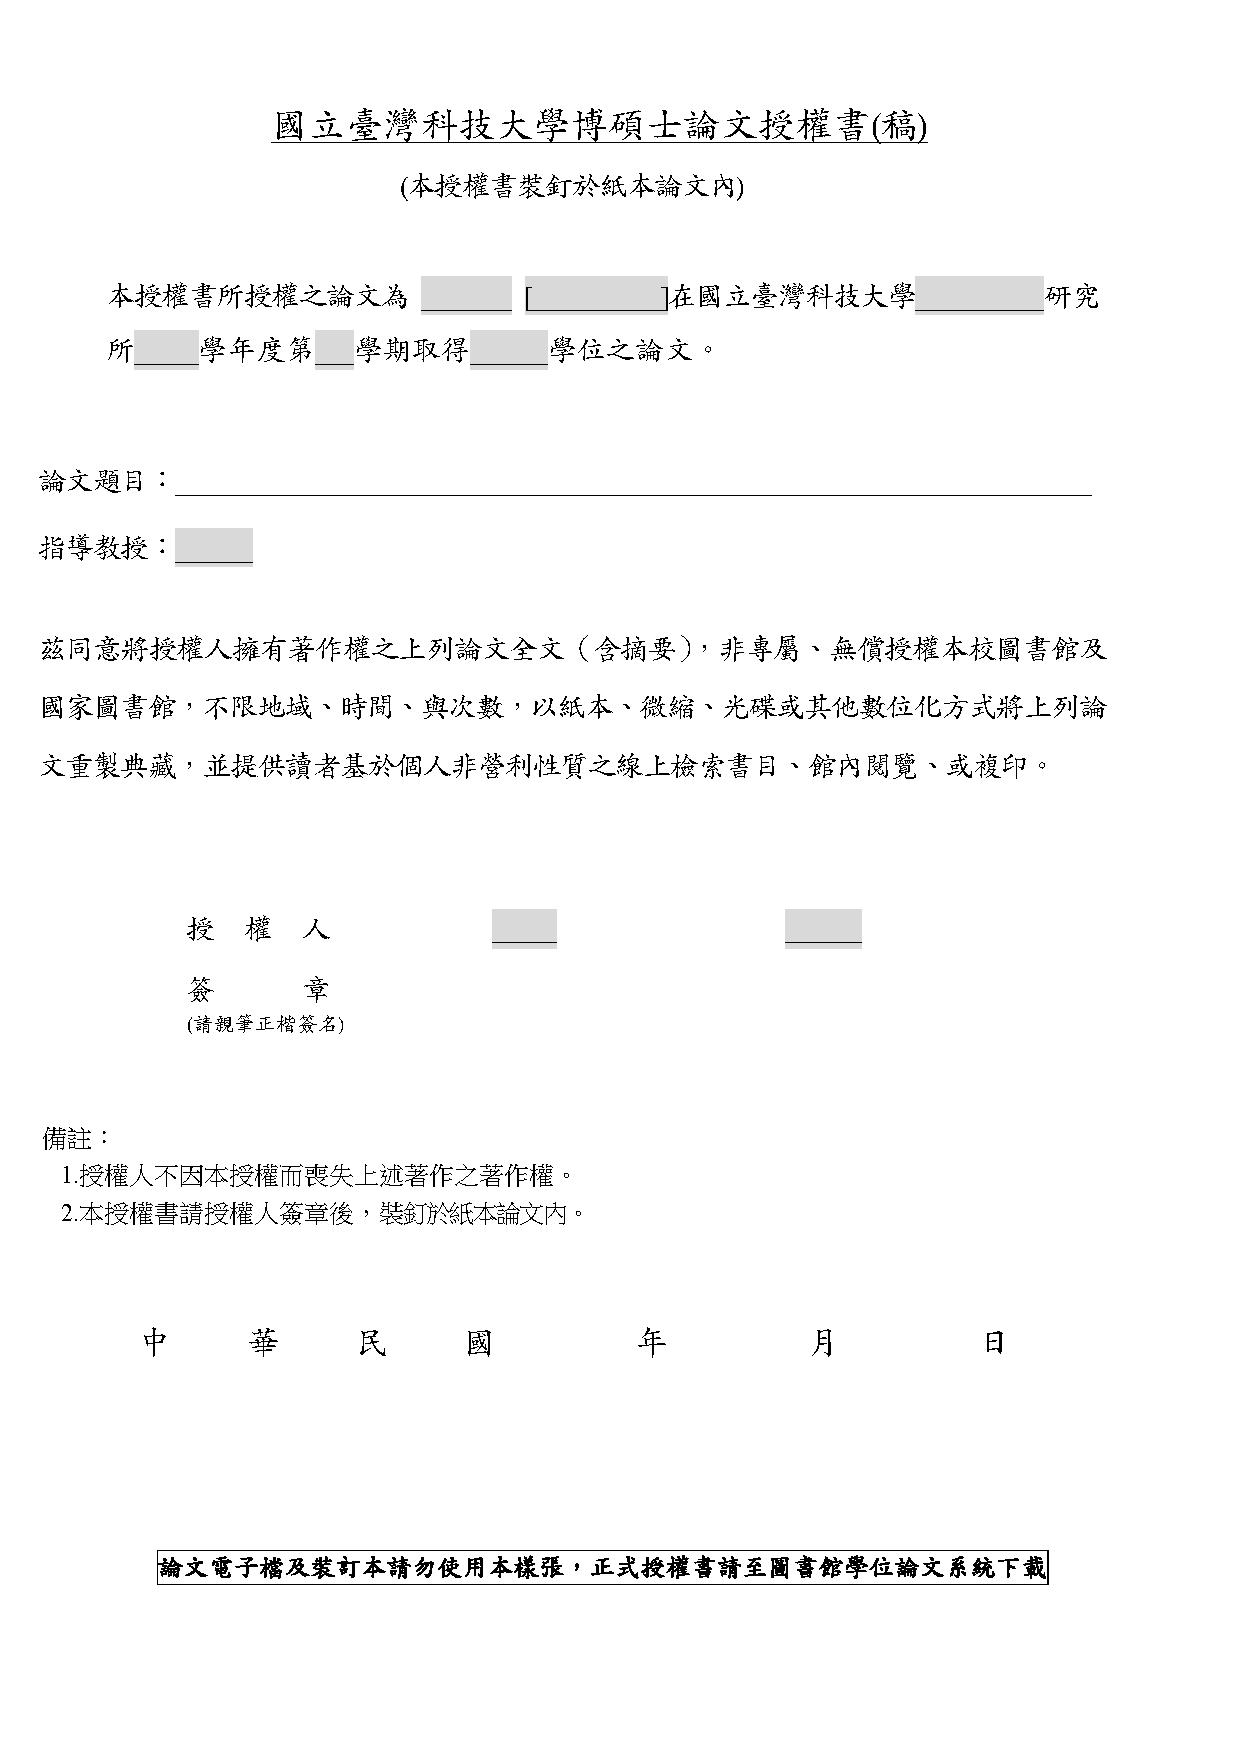
\includegraphics[width=9cm]{a}
  \caption{fig}
\end{figure}
\begin{figure}[H]
  \centering
  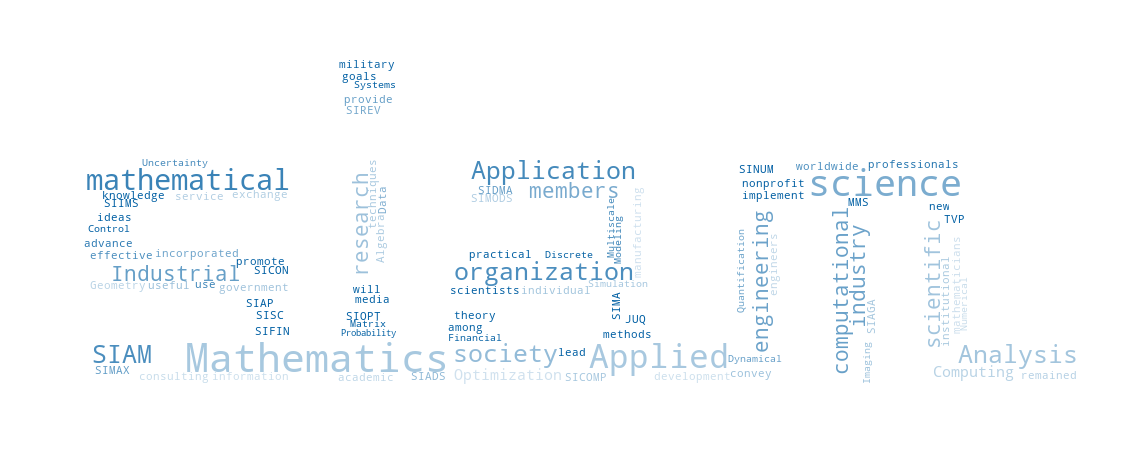
\includegraphics[width=9cm]{b}
  \caption{sfd}
\end{figure}
\begin{table}[H]
  \centering
  \begin{tabular}{rl}
    a&ads
  \end{tabular}
  \caption{as}
\end{table}
\begin{table}[H]
  \centering
  \begin{tabular}{rl}
    a&ads
  \end{tabular}
  \caption{as}
\end{table}

\begin{table}[H]
  \centering
  \begin{tabular}{rl}
    a&ads
  \end{tabular}
  \caption{asasd}
\end{table}
\begin{Algorithm}[H]
    \SetKwFunction{Sum}{sum} % use to define a function name
    \BlankLine
    \Input{Parameters: $i$.}
    \Output{Result: $s$.}
    \BlankLine
    $I\gets \{1,2,3,\ldots,100\}$ \;
    \BlankLine
    \ForEach{$i\in I$}
    {%
        $L_i \gets i$ \;
        $M_i \gets e^i$ \;
    }
    \BlankLine
    \For{$i=1$ \KwTo $100$}
    {%
         $p^i \gets \Sum( l_i,M_i)$ \;
        \If{$i$ is even}
        {%
            $p_i\gets p_i-1$ \;
        }
    }
    \BlankLine
    \For{$i=1: 100$}
    {%
        $q^i \gets \Sum(e^{l_i},e^{M_i})$ \;
        \If{$i$ is even}
        {%
            $q_i\gets p_i-1$ \;
        }
    }
    \While{$i\neq 2$}{$i=i+1$}
     $s\gets p^i+q^i$
    \caption{A example of the algorithms}
    \label{algo:Ch6-ShapeGen}
\end{Algorithm}
\lstinputlisting[language=Matlab,caption={matlab code}]{nearest_product.m}  %% donot need add the parentpath
%%% Local Variables:
%%% mode: latex
%%% TeX-master: "thesis"
%%% End: